\graphicspath{{chapt_dutch/}{intro/}{chapt2/}{chapt3/}{chapt4/}{chapt5/}{chapt6/}{chapt7/}}

% Header
\renewcommand\evenpagerightmark{{\scshape\small Appendix A}}
\renewcommand\oddpageleftmark{{\scshape\small A data acquisition software for VME CAEN TDCs}}

\renewcommand{\bibname}{References}

\hyphenation{}

\chapter[A data acquisition software for VME CAEN TDCs]%
{A data acquisition software for VME CAEN TDCs}
\label{app1}

Certifying detectors in the perspective of HL-LHC required to develop tools for the GIF++ experiment. One of them was the \acf{DAQ} software that allows to make the communications in between the computer and the TDC modules in order to retrieve the RPC data~\cite{GIFDAQ}. In this appendix, details about the software, as of how the software was written, how it functions and how it can be exported to another similar setup.

\section{Description of the setup}

	As previously described in Section~\ref{ssec:PulseProc}, CMS RPC FEEs provide us with \SI{100}{ns} long LVDS output signals. These signals are then sent into V1190A \acf{TDC} modules manufactured by CAEN~\cite{V1190AMUT}. V1190A are VME units accepting 128 independent Multi-Hit/Multi-Event TDC channels whose signals are treated by 4 \SI{100}{ps} high performance TDC chips, developped by CERN/ECP-MIC Division. The data acquisition used at GIF takes profit of the \textit{Trigger Matching Mode} offered by modules V1190A. A trigger matching is performed in between a trigger time tag and the channel time measurements. The signal provided by the coïncidence of both PMTs is used to trigger the data acquisition. Control over this data acquisition mode, explained through Figure~\ref{fig:V1190A-TMM} is offered through 4 programmable parameters:
        
	\begin{itemize}
		\item \textbf{match window:} the match between a trigger and a hit is done within a programmable time window
		\item \textbf{window offset:} temporal distance between the trigger tag and the start of the trigger matching window
		\item \textbf{extra search margin:} an extended time window is used to ensure that all matching hits are found
		\item \textbf{reject margin:} older hits are automatically rejected to preven buffer overflows and to speed up the search time
	\end{itemize}
    
    \begin{figure}
		\centering
		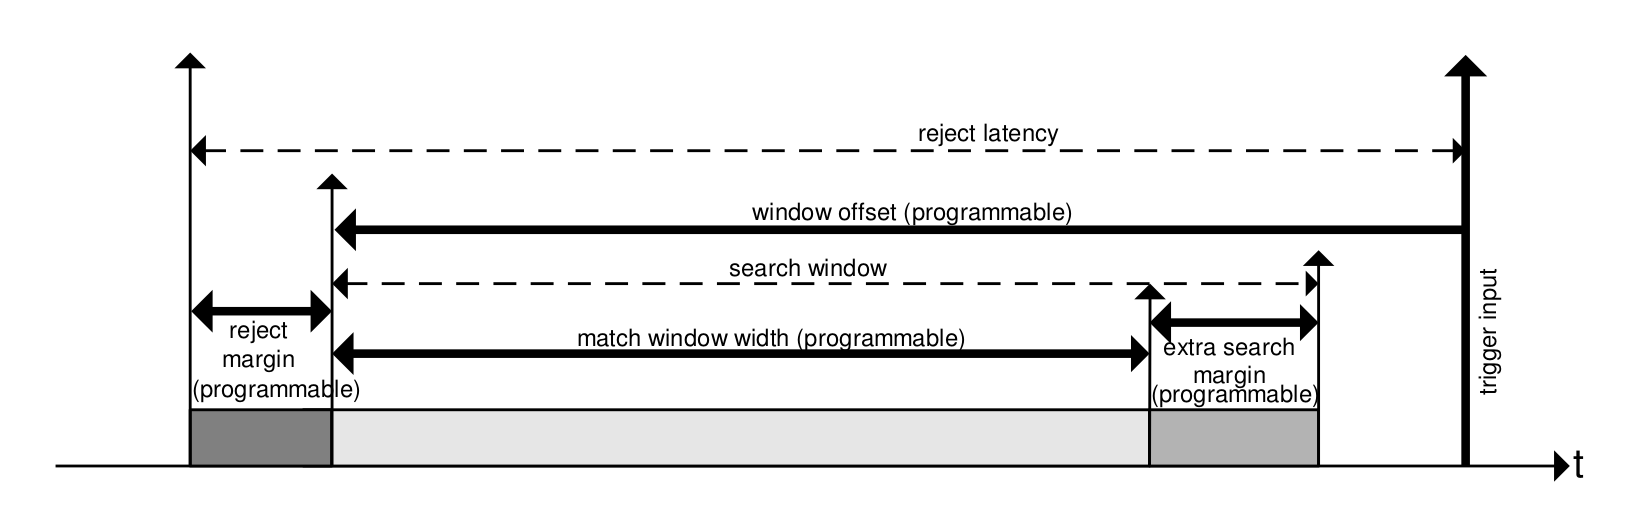
\includegraphics[width = 1.25\plotwidth]{fig/chapt5/V1190A-TMM.png}\\
		\caption{\label{fig:V1190A-TMM} Module V1190A \textit{Trigger Matching Mode} timing diagram.}
	\end{figure}
	
	The communication between the computer ond the TDCs to transfer data is done via a V1718 VME master module operated from a USB port. 

\section{Data read-out}

\section{Software export}


\clearpage{\pagestyle{empty}\cleardoublepage}
